% !TEX spellcheck = en_US



% ~~~~~~~~~~~~~~~~~~~~~~~~~~~~~~~~~~~~~~~ V
% (NC) 2026 Haluk Bingol
% github.com/halukbingol/LaTeX-Templates
%
% Licensees may copy, distribute, display, and perform the work and make derivative works 
% and remixes based on it only for non-commercial purposes. 
% ~~~~~~~~~~~~~~~~~~~~~~~~~~~~~~~~~~~~~~~ A


% v20261029T1800

\documentclass[aspectratio=169,10pt,compress]{beamer}




% ~~~~~~~~~~~~~~~~~~~~~~~~~~~~~~~~~~~~~~~~~~~~~~~~~~~~~~~~~~~~~~~~~ V hblib
	\usepackage{../../hblib/hblibPresentation} % lib presentation: theme, i/N, \hSection, algorithm2e, ...
	\usepackage{../../hblib/hblibCodeoutput} % lib code + output: \lstcode, \lstterminal, ...
	\usepackage{../../hblib/hblibDatastructures} % lib data structures: \hString, \hStack, \hQueue, \hArray
% ~~~~~~~~~~~~~~~~~~~~~~~~~~~~~~~~~~~~~~~~~~~~~~~~~~~~~~~~~~~~~~~~~ A hblib




% +++++++++++++++++++++++++++++++++++++++ V specific
\DontPrintSemicolon % in algorithms
% +++++++++++++++++++++++++++++++++++++++ A specific



\title[Arrays 1D: Concepts]{
	One-Dimensional Arrays\\
	Concepts
}
\subtitle{
	\cisOOO\ -- Level 0: ideas and pictures
}
\author[Erkovan]{Sait Erkovan}

\institute[FCIS]{
	Faculty of Computer and Information Sciences\\
	Yeditepe University
}
\date{{\tiny \hbTimeStamp}}

\begin{document}




% ~~~~~~~~~~~~~~~~~~~~~~~~~~~~~~~~~~~~~~ V frm
\begin{frame}[t,fragile]
	\titlepage
\end{frame}
% ~~~~~~~~~~~~~~~~~~~~~~~~~~~~~~~~~~~~~~ A frm




% ~~~~~~~~~~~~~~~~~~~~~~~~~~~~~~~~~~~~~~ V frm
\begin{frame}[t,fragile] \frametitle{Outline}
	\begin{columns}[T]
		\begin{column}{0.48\textwidth}
			\tableofcontents[sections={1-4}, hideallsubsections]
		\end{column}
		\begin{column}{0.48\textwidth}
			\tableofcontents[sections={5-8}, hideallsubsections]
		\end{column}
	\end{columns}

	\vspace{1em}
	\small This deck has ideas, pictures and pseudo code only.
	The same ideas as Java programs: \hCode{array1D-5-examples}.
\end{frame}
% ~~~~~~~~~~~~~~~~~~~~~~~~~~~~~~~~~~~~~~ A frm




% ~~~~~~~~~~~~~~~~~~~~~~~~~~~~~~~~~~~~~~ V
\hSection[Why]{Why arrays?}
% ~~~~~~~~~~~~~~~~~~~~~~~~~~~~~~~~~~~~~~ A




% ~~~~~~~~~~~~~~~~~~~~~~~~~~~~~~~~~~~~~~ V frm
\begin{frame}[t,fragile] \frametitle{Many values of the same kind}
	Daily high temperatures of one week in Istanbul.

	\begin{columns}[T]
		\begin{column}{0.40\textwidth}
			\textbf{Seven variables}

			\vspace{0.5em}
			\begin{tikzpicture}
				\foreach \v [count=\k from 0] in {14.0,16.5,13.0,18.5,17.0,12.5,13.5} {
					\node[hvar, minimum width=1.0cm] (t\k) at ({mod(\k,4)*1.45}, {-floor(\k/4)*1.1}) {\v};
					\node[font=\ttfamily\scriptsize, above=0pt of t\k] {t\k};
				}
			\end{tikzpicture}
		\end{column}
		\begin{column}{0.56\textwidth}
			\textbf{One array}

			\vspace{1.2em}
			\begin{tikzpicture}
				\hArray[id=h, name=highs, width=0.85]{14.0,16.5,13.0,18.5,17.0,12.5,13.5}
			\end{tikzpicture}
		\end{column}
	\end{columns}

	\vspace{1em}
	\begin{itemize}
		\item Seven names, or \hEmph{one name and a number}: \hCode{highs[3]} is the fourth day
		\item The number can be \hEmph{computed}: \hCode{highs[i]}, \hCode{highs[i + 1]}
		\item So \hEmph{one loop} can visit every day; no loop can visit \hCode{t0}, \hCode{t1}, \dots
	\end{itemize}
\end{frame}
% ~~~~~~~~~~~~~~~~~~~~~~~~~~~~~~~~~~~~~~ A frm




% ~~~~~~~~~~~~~~~~~~~~~~~~~~~~~~~~~~~~~~ V frm
\begin{frame}[t,fragile] \frametitle{Questions that need memory}
	\hQuestion{Which days were warmer than the week's average?}

	\begin{enumerate}
		\item Look at all seven values to get the average
		\item Look at all seven values \hEmph{again} to compare them with the average
	\end{enumerate}
	The values are needed twice, so they must be \hDefined{kept}.

	\vspace{0.5em}


% +++++++++++++++++++++++++++++++++++++++ V tbl
%: -Tbl. need to keep
\begin{table}
		\small
		\begin{tabular}{@{}L{0.42\textwidth}L{0.18\textwidth}L{0.32\textwidth}@{}}
			\toprule
			\textbf{Question about a sequence} & \textbf{Keep all?} & \textbf{Why} \\
			\midrule
			Sum of the values             & no  & one running total is enough \\
			Largest value                 & no  & keep only the best so far \\
			Values above the average      & yes & the average is known only at the end \\
			Print them in reverse order   & yes & the last one is printed first \\
			The middle value (median)     & yes & needs the values in order \\
			\bottomrule
		\end{tabular}
\end{table}%
% +++++++++++++++++++++++++++++++++++++++ A tbl
\end{frame}
% ~~~~~~~~~~~~~~~~~~~~~~~~~~~~~~~~~~~~~~ A frm




% ~~~~~~~~~~~~~~~~~~~~~~~~~~~~~~~~~~~~~~ V
\hSection[Anatomy]{Anatomy of an array}
% ~~~~~~~~~~~~~~~~~~~~~~~~~~~~~~~~~~~~~~ A




% ~~~~~~~~~~~~~~~~~~~~~~~~~~~~~~~~~~~~~~ V frm
\begin{frame}[t,fragile] \frametitle{The parts of an array}
	\begin{center}
		\begin{tikzpicture}
			\hArray[id=h, name=highs, width=1.0, hot={3}]{14.0,16.5,13.0,18.5,17.0,12.5,13.5}
			\node[colorIndex, font=\small, align=center] (ix) at (3.5,1.5) {index 3};
			\draw[->, colorIndex] (ix) -- (3.5,0.68);
			\node[font=\small] (el) at (6.3,1.5) {element \hCode{highs[3]} is 18.5};
			\draw[->] (el.south west) -- (h-3.north east);
			\draw[decorate, decoration={brace, mirror, amplitude=5pt}] (0,-0.12) -- (7,-0.12)
				node[midway, below=6pt, font=\small] {length 7: \hCode{highs.length}};
		\end{tikzpicture}
	\end{center}


% +++++++++++++++++++++++++++++++++++++++ V tbl
%: -Tbl. parts
\begin{table}
		\small
		\begin{tabular}{@{}L{0.18\textwidth}L{0.46\textwidth}L{0.28\textwidth}@{}}
			\toprule
			\textbf{Term} & \textbf{Meaning} & \textbf{In Java} \\
			\midrule
			element      & one stored value                         & \hCode{highs[3]} \\
			index        & the position of an element: $0, 1, \dots, n - 1$ & \hCode{3}, \hCode{i} \\
			length $n$   & how many elements there are              & \hCode{highs.length} \\
			element type & the type of \emph{every} element         & \hCode{double} \\
			\bottomrule
		\end{tabular}
\end{table}%
% +++++++++++++++++++++++++++++++++++++++ A tbl
\end{frame}
% ~~~~~~~~~~~~~~~~~~~~~~~~~~~~~~~~~~~~~~ A frm




% ~~~~~~~~~~~~~~~~~~~~~~~~~~~~~~~~~~~~~~ V frm
\begin{frame}[t,fragile] \frametitle{Why the first index is 0}
	\begin{columns}[T]
		\begin{column}{0.52\textwidth}
			The elements sit \hEmph{side by side} in memory.
			The index says how many elements to \hEmph{skip} from the start.

			\vspace{0.5em}
			If the array starts at address $s$ and one element takes $b$ bytes:
			\[
				\mathit{address}(i) = s + i \cdot b
			\]
			The first element skips nothing: $i = 0$.
			\cite{knuth1973artv1}

			\vspace{0.5em}
			\hRemark{Valid indices:}
			\[
				0 \le i \le n - 1
				\qquad \text{that is} \qquad
				0 \le i < n
			\]
		\end{column}
		\begin{column}{0.44\textwidth}
			An \hCode{int} takes 4 bytes; $s = 1000$:

			\vspace{0.5em}
			\begin{tikzpicture}
				\hArray[id=m, width=1.1, height=0.55]{85,72,0,90}
				\foreach \k in {0,...,3} {
					\pgfmathtruncatemacro{\adr}{1000 + 4*\k}
					\node[font=\scriptsize\ttfamily, below=2pt of m-\k] {\adr};
				}
				\node[font=\scriptsize, anchor=east] at (-0.1,-0.25) {address};
			\end{tikzpicture}

			\vspace{1em}
			\small Element 3 is at $1000 + 3 \cdot 4 = 1012$:
			one multiplication, one addition, \hEmph{no matter how long} the array is.
		\end{column}
	\end{columns}
\end{frame}
% ~~~~~~~~~~~~~~~~~~~~~~~~~~~~~~~~~~~~~~ A frm




% ~~~~~~~~~~~~~~~~~~~~~~~~~~~~~~~~~~~~~~ V frm
\begin{frame}[t,fragile] \frametitle{Length is a count, index is a position}
	\begin{center}
		\begin{tikzpicture}
			\hArray[id=a, width=1.0, hot={4}, unused={}]{a,b,c,d,e}
			\node[hvar, draw=colorStop, dashed, text=colorStop] (out) at (5.5,0.25) {?};
			\node[colorIndex, font=\tiny] at (5.5,0.64) {5};
			\node[font=\small, align=left, anchor=west] at (6.2,0.25) {no element 5:\\ \hCode{n = 5} is \emph{not} an index};
			\node[font=\small] at (4.5,-0.45) {last index $n - 1 = 4$};
		\end{tikzpicture}
	\end{center}

	\begin{columns}[T]
		\begin{column}{0.48\textwidth}
			\textbf{Counting from 1 (everyday)}
			\begin{itemize}
				\item first, second, \dots, fifth
				\item the last one is number $n$
			\end{itemize}
		\end{column}
		\begin{column}{0.48\textwidth}
			\textbf{Counting from 0 (arrays)}
			\begin{itemize}
				\item index $0, 1, \dots, 4$
				\item the last one is index $n - 1$
			\end{itemize}
		\end{column}
	\end{columns}

	\vspace{0.5em}
	\begin{alertblock}{Off by one}
		Using $n$ as an index, starting at 1, or stopping at $i \le n$ instead of $i < n$
		are the most common array mistakes. Java stops the program when an index is outside
		$0 \dots n - 1$.
	\end{alertblock}
\end{frame}
% ~~~~~~~~~~~~~~~~~~~~~~~~~~~~~~~~~~~~~~ A frm




% ~~~~~~~~~~~~~~~~~~~~~~~~~~~~~~~~~~~~~~ V
\hSection[Rules]{The rules of a Java array}
% ~~~~~~~~~~~~~~~~~~~~~~~~~~~~~~~~~~~~~~ A




% ~~~~~~~~~~~~~~~~~~~~~~~~~~~~~~~~~~~~~~ V frm
\begin{frame}[t,fragile] \frametitle{One type, fixed length}


% +++++++++++++++++++++++++++++++++++++++ V tbl
%: -Tbl. rules
\begin{table}
		\small
		\begin{tabular}{@{}L{0.22\textwidth}L{0.34\textwidth}L{0.36\textwidth}@{}}
			\toprule
			\textbf{Rule} & \textbf{Meaning} & \textbf{So \dots} \\
			\midrule
			One element type & all elements are \hCode{int}, or all are \hCode{String}, \dots
			                 & mixed data (name \emph{and} score) needs two arrays or objects \\
			Fixed length     & chosen when the array is created; never changes
			                 & to ``grow'', make a bigger array and copy \\
			Numbered slots   & every slot exists from the start, with a value
			                 & there are no ``holes'', only values you do not use \\
			\bottomrule
		\end{tabular}
\end{table}%
% +++++++++++++++++++++++++++++++++++++++ A tbl


	\begin{center}
		\begin{tikzpicture}
			\hArray[id=s, name={scores}, width=0.8]{85,72,90}
			\node[font=\small, anchor=west] at (2.7,0.25) {3 slots, forever};
			\hArray[id=t, name={bigger}, at={(6.6,0)}, width=0.8, hot={0,1,2}, unused={3,4,5}]{85,72,90,0,0,0}
			\node[font=\scriptsize, anchor=north] at (8.0,-0.15) {copied};
			\node[font=\scriptsize, anchor=north] at (10.4,-0.15) {room to grow};
		\end{tikzpicture}
	\end{center}
\end{frame}
% ~~~~~~~~~~~~~~~~~~~~~~~~~~~~~~~~~~~~~~ A frm




% ~~~~~~~~~~~~~~~~~~~~~~~~~~~~~~~~~~~~~~ V frm
\begin{frame}[t,fragile] \frametitle{Every slot starts with a default value}
	\begin{columns}[T]
		\begin{column}{0.46\textwidth}


% +++++++++++++++++++++++++++++++++++++++ V tbl
%: -Tbl. default values
\begin{table}
				\small
				\begin{tabular}{@{}ll@{}}
					\toprule
					\textbf{Element type} & \textbf{Starts as} \\
					\midrule
					\hCode{int}, \hCode{long}     & \hCode{0} \\
					\hCode{double}                & \hCode{0.0} \\
					\hCode{boolean}               & \hCode{false} \\
					\hCode{char}                  & the character with code 0 \\
					\hCode{String}, any object    & \hCode{null}: \emph{no object} \\
					\bottomrule
				\end{tabular}
\end{table}%
% +++++++++++++++++++++++++++++++++++++++ A tbl
		\end{column}
		\begin{column}{0.48\textwidth}
			\vspace{0.6em}
			\begin{tikzpicture}
				\hArray[id=c, name={counts}, width=0.8]{0,0,0,0}
				\hArray[id=p, name={present}, at={(0,-1.1)}, width=0.95, font=\ttfamily\scriptsize]{false,false,false}
				\hArray[id=n, name={names}, at={(0,-2.2)}, width=0.95, font=\ttfamily\scriptsize]{null,null,null}
			\end{tikzpicture}
		\end{column}
	\end{columns}

	\vspace{1em}
	\begin{itemize}
		\item A new array is never ``empty'': every element has a value from the start
		\item \hCode{null} in a \hCode{String} array means ``no string here yet'';
		      using it as a string stops the program
	\end{itemize}
\end{frame}
% ~~~~~~~~~~~~~~~~~~~~~~~~~~~~~~~~~~~~~~ A frm




% ~~~~~~~~~~~~~~~~~~~~~~~~~~~~~~~~~~~~~~ V
\hSection[Memory]{Arrays live in memory}
% ~~~~~~~~~~~~~~~~~~~~~~~~~~~~~~~~~~~~~~ A




% ~~~~~~~~~~~~~~~~~~~~~~~~~~~~~~~~~~~~~~ V frm
\begin{frame}[t,fragile] \frametitle{The variable holds a reference}
	\begin{center}
		\begin{tikzpicture}
			\draw[rounded corners, gray!60, dashed] (2.2,-0.6) rectangle (9.0,1.2);
			\node[gray, font=\scriptsize, anchor=north east] at (9.0,1.2) {memory for objects (heap)};
			\hArray[id=h, at={(3.0,0)}, width=0.75]{14.0,16.5,13.0,18.5,17.0,12.5,13.5}
			\node[hvar] (v) at (0.6,0.25) {};
			\node[font=\ttfamily\small, left=2pt of v] {highs};
			\draw[href] (v.center) -- (h-0.west);
		\end{tikzpicture}
	\end{center}

	\begin{itemize}
		\item Creating an array puts the elements \hEmph{somewhere} in memory
		\item The variable does not contain the elements; it contains \hDefined{where they are}:
		      a \hDefined{reference} (drawn as an arrow)
		\item \hCode{null} is the reference to \emph{no} array
	\end{itemize}

	\begin{block}{Why it matters}
		Copying the variable copies the \emph{arrow}, not the elements.
		The next two slides show what follows from this.
	\end{block}
\end{frame}
% ~~~~~~~~~~~~~~~~~~~~~~~~~~~~~~~~~~~~~~ A frm




% ~~~~~~~~~~~~~~~~~~~~~~~~~~~~~~~~~~~~~~ V frm
\begin{frame}[t,fragile] \frametitle{Two names, one array: aliasing}
	\begin{center}
		\begin{tikzpicture}
			\only<1-2>{\hArray[id=x, at={(3,0)}, width=0.8]{1,2,3}}
			\only<3>{\hArray[id=x, at={(3,0)}, width=0.8, hot={0}]{99,2,3}}
			\node[hvar] (a) at (0.6,0.6) {};
			\node[font=\ttfamily\small, left=2pt of a] {a};
			\draw[href] (a.center) -- (x-0.west);
			\uncover<2->{
				\node[hvar] (b) at (0.6,-0.4) {};
				\node[font=\ttfamily\small, left=2pt of b] {b};
				\draw[href] (b.center) -- (x-0.south west);
			}
		\end{tikzpicture}
	\end{center}


% +++++++++++++++++++++++++++++++++++++++ V tbl
%: -Tbl. aliasing steps
\begin{table}
		\small
		\begin{tabular}{@{}lL{0.62\textwidth}@{}}
			\toprule
			\textbf{Step} & \textbf{Picture} \\
			\midrule
			\hCode{a} refers to \{1, 2, 3\}   & one arrow \\
			\hCode{b = a}     & a \emph{second arrow} to the \emph{same} array; nothing is copied \\
			\hCode{b[0] = 99} & the one array changes, so \hCode{a[0]} is 99, too \\
			\bottomrule
		\end{tabular}
\end{table}%
% +++++++++++++++++++++++++++++++++++++++ A tbl
\end{frame}
% ~~~~~~~~~~~~~~~~~~~~~~~~~~~~~~~~~~~~~~ A frm




% ~~~~~~~~~~~~~~~~~~~~~~~~~~~~~~~~~~~~~~ V frm
\begin{frame}[t,fragile] \frametitle{A copy is a second array}
	\begin{center}
		\begin{tikzpicture}
			\hArray[id=x, at={(3,0)}, width=0.8]{1,2,3}
			\hArray[id=y, at={(3,-1.2)}, width=0.8, hot={1}]{1,77,3}
			\node[hvar] (a) at (0.6,0.25) {};
			\node[font=\ttfamily\small, left=2pt of a] {a};
			\draw[href] (a.center) -- (x-0.west);
			\node[hvar] (c) at (0.6,-0.95) {};
			\node[font=\ttfamily\small, left=2pt of c] {c};
			\draw[href] (c.center) -- (y-0.west);
			\node[font=\small, anchor=west] at (5.8,-0.95) {new array, elements copied one by one, then \hCode{c[1] = 77}};
		\end{tikzpicture}
	\end{center}


% +++++++++++++++++++++++++++++++++++++++ V tbl
%: -Tbl. same array or same contents
\begin{table}
		\small
		\begin{tabular}{@{}L{0.36\textwidth}L{0.56\textwidth}@{}}
			\toprule
			\textbf{Question} & \textbf{Answer} \\
			\midrule
			Same array? (same arrow)           & \hCode{a == b} is \hCode{true} only for aliases \\
			Same contents? (same elements)    & compare element by element; \hCode{a == c} is \hCode{false} \\
			Change one, see it in the other?  & aliases: yes \quad copies: no \\
			\bottomrule
		\end{tabular}
\end{table}%
% +++++++++++++++++++++++++++++++++++++++ A tbl
\end{frame}
% ~~~~~~~~~~~~~~~~~~~~~~~~~~~~~~~~~~~~~~ A frm




% ~~~~~~~~~~~~~~~~~~~~~~~~~~~~~~~~~~~~~~ V
\hSection[Patterns]{Thinking in traversals}
% ~~~~~~~~~~~~~~~~~~~~~~~~~~~~~~~~~~~~~~ A




% ~~~~~~~~~~~~~~~~~~~~~~~~~~~~~~~~~~~~~~ V frm
\begin{frame}[t,fragile] \frametitle{Visiting every element}
	A \hDefined{traversal} visits the elements one by one, by index.

	\begin{center}
		\begin{tikzpicture}
			\only<1>{\hArray[id=a, name={a}, width=0.9, cur={0}]{72,85,90,64,78}}
			\only<2>{\hArray[id=a, name={a}, width=0.9, done={0}, cur={1}]{72,85,90,64,78}}
			\only<3>{\hArray[id=a, name={a}, width=0.9, done={0,1}, cur={2}]{72,85,90,64,78}}
			\only<4>{\hArray[id=a, name={a}, width=0.9, done={0,...,2}, cur={3}]{72,85,90,64,78}}
			\only<5>{\hArray[id=a, name={a}, width=0.9, done={0,...,3}, cur={4}]{72,85,90,64,78}}
			\only<6>{\hArray[id=a, name={a}, width=0.9, done={0,...,4}]{72,85,90,64,78}}
			\foreach \k in {0,...,5} {
				\only<\the\numexpr\k+1\relax>{\node[font=\ttfamily\small, colorTop!60!black] at (\k*0.9+0.45,-0.45) {i = \k};}
			}
			\only<6>{\node[font=\small, anchor=west] at (5.0,0.25) {$i = 5 = n$: stop};}
		\end{tikzpicture}
	\end{center}

	\begin{columns}[T]
		\begin{column}{0.48\textwidth}


% +++++++++++++++++++++++++++++++++++++++ V alg
%: -Alg. traversal
\begin{algorithm}[H]
				\caption{Traverse($a$)}
				$i \gets 0$\;
				\While{$i < n$}{
					visit $a[i]$\;
					$i \gets i + 1$\;
				}
\end{algorithm}
% +++++++++++++++++++++++++++++++++++++++ A alg

		\end{column}
		\begin{column}{0.48\textwidth}
			\begin{itemize}\small
				\item Start at index 0
				\item Continue while $i < n$
				\item The same skeleton for every pattern on the next slides;
				      only ``visit'' changes
			\end{itemize}
		\end{column}
	\end{columns}
\end{frame}
% ~~~~~~~~~~~~~~~~~~~~~~~~~~~~~~~~~~~~~~ A frm




% ~~~~~~~~~~~~~~~~~~~~~~~~~~~~~~~~~~~~~~ V frm
\begin{frame}[t,fragile] \frametitle{A catalogue of traversal patterns}


% +++++++++++++++++++++++++++++++++++++++ V tbl
%: -Tbl. patterns
\begin{table}
		\footnotesize
		\begin{tabular}{@{}L{0.12\textwidth}L{0.21\textwidth}L{0.13\textwidth}L{0.23\textwidth}L{0.12\textwidth}@{}}
			\toprule
			\textbf{Pattern} & \textbf{Question} & \textbf{Start} & \textbf{At element $i$} & \textbf{Result} \\
			\midrule
			Fill        & set every element         & --                      & $a[i] \gets f(i)$                         & filled array \\
			Accumulate  & total? average?           & $s \gets 0$             & $s \gets s + a[i]$                        & $s$, $s / n$ \\
			Best so far & largest? smallest?        & $b \gets 0$ (an index)  & if $a[i] > a[b]$: $b \gets i$             & $b$, $a[b]$ \\
			Search      & where is the first match? & $p \gets 0$             & stop at the first match                   & $p$ or $-1$ \\
			Count       & how many match?           & $c \gets 0$             & if match: $c \gets c + 1$                 & $c$ \\
			Transform   & change every element      & --                      & $a[i] \gets g(a[i])$                      & same array \\
			Filter      & the matches, as an array  & count first             & copy the matches                          & new array \\
			\bottomrule
		\end{tabular}
\end{table}%
% +++++++++++++++++++++++++++++++++++++++ A tbl


	\vspace{0.3em}
	\begin{itemize}\small
		\item Most array problems are one pattern, or two patterns in one loop
		\item Name the pattern first, then write the loop
	\end{itemize}
\end{frame}
% ~~~~~~~~~~~~~~~~~~~~~~~~~~~~~~~~~~~~~~ A frm




% ~~~~~~~~~~~~~~~~~~~~~~~~~~~~~~~~~~~~~~ V frm
\begin{frame}[t,fragile] \frametitle{Accumulate: total and average}
	\begin{columns}[T]
		\begin{column}{0.48\textwidth}
			\SetAlFnt{\small}


% +++++++++++++++++++++++++++++++++++++++ V alg
%: -Alg. average
\begin{algorithm}[H]
				\caption{Average($a$)}
				\KwIn{array $a$ of $n$ numbers}
				$s \gets 0$\;
				\For{$i \gets 0$ \KwTo $n - 1$}{
					$s \gets s + a[i]$\;
				}
				\eIf{$n > 0$}{
					\Return{$s / n$}\;
				}{
					\Return{undefined}\;
				}
\end{algorithm}
% +++++++++++++++++++++++++++++++++++++++ A alg

		\end{column}
		\begin{column}{0.48\textwidth}
			\begin{center}
				\begin{tikzpicture}
					\hArray[id=a, width=0.8, done={0,...,4}]{72,85,90,64,78}
				\end{tikzpicture}
			\end{center}
			\begin{itemize}\small
				\item $s$: $0 \to 72 \to 157 \to 247 \to 311 \to 389$
				\item average $389 / 5 = 77.8$
				\item \hRemark{Empty array}: $n = 0$, so $s / n$ has no meaning.
				      Decide what to do \emph{before} you divide.
				\item Integer division: $389 / 5$ is 77 in Java unless one side is a \hCode{double}
			\end{itemize}
		\end{column}
	\end{columns}
\end{frame}
% ~~~~~~~~~~~~~~~~~~~~~~~~~~~~~~~~~~~~~~ A frm




% ~~~~~~~~~~~~~~~~~~~~~~~~~~~~~~~~~~~~~~ V frm
\begin{frame}[t,fragile] \frametitle{Best so far: largest and smallest}
	\begin{columns}[T]
		\begin{column}{0.48\textwidth}
			\SetAlFnt{\small}


% +++++++++++++++++++++++++++++++++++++++ V alg
%: -Alg. best so far
\begin{algorithm}[H]
				\caption{IndexOfMax($a$), $n \ge 1$}
				$b \gets 0$ \tcp*{the best is the first}
				\For{$i \gets 1$ \KwTo $n - 1$}{
					\If{$a[i] > a[b]$}{
						$b \gets i$\;
					}
				}
				\Return{$b$}\;
\end{algorithm}
% +++++++++++++++++++++++++++++++++++++++ A alg

		\end{column}
		\begin{column}{0.48\textwidth}
			\begin{center}
				\begin{tikzpicture}
					\only<1>{\hArray[id=a, width=0.8, hot={0}]{-5,-2,-9,-2}}
					\only<2>{\hArray[id=a, width=0.8, done={0}, hot={1}]{-5,-2,-9,-2}}
					\only<3->{\hArray[id=a, width=0.8, done={0,2,3}, hot={1}]{-5,-2,-9,-2}}
				\end{tikzpicture}
			\end{center}
			\begin{itemize}\small
				\item Keep the \hEmph{index} of the best: you get its value \emph{and} where it is
				\item Start with the \hEmph{first element}, not with 0: with all negative
				      values, 0 would ``win'' although it is not in the array
				\item \uncover<3->{$>$ keeps the \emph{first} of equal values; $\ge$ would keep the last}
				\item Smallest: the same with $<$
			\end{itemize}
		\end{column}
	\end{columns}
\end{frame}
% ~~~~~~~~~~~~~~~~~~~~~~~~~~~~~~~~~~~~~~ A frm




% ~~~~~~~~~~~~~~~~~~~~~~~~~~~~~~~~~~~~~~ V frm
\begin{frame}[t,fragile] \frametitle{Search: where is the first match?}
	\begin{columns}[T]
		\begin{column}{0.48\textwidth}
			\SetAlFnt{\small}


			\SetKw{KwAnd}{and}
			\SetKw{KwNot}{not}


% +++++++++++++++++++++++++++++++++++++++ V alg
%: -Alg. linear search
\begin{algorithm}[H]
				\caption{LinearSearch($a$, $x$)}
				$p \gets 0$; \quad $\mathit{found} \gets$ false\;
				\While{$p < n$ \KwAnd \KwNot $\mathit{found}$}{
					\eIf{$a[p] = x$}{
						$\mathit{found} \gets$ true\;
					}{
						$p \gets p + 1$\;
					}
				}
				\lIf{$\mathit{found}$}{\Return{$p$}}
				\Return{$-1$} \tcp*{$-1$ is never an index}
\end{algorithm}
% +++++++++++++++++++++++++++++++++++++++ A alg

		\end{column}
		\begin{column}{0.48\textwidth}
			\begin{center}
				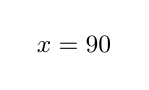
\begin{tikzpicture}
					\hArray[id=a, width=0.8, done={0,1}, hot={2}]{72,85,90,64,90}
					\node[font=\small, anchor=west] at (4.2,0.25) {$x = 90$};
				\end{tikzpicture}
			\end{center}
			\begin{itemize}\small
				\item Stops at the \hEmph{first} match: index 2, not 4
				\item Not found: every element was checked, all $n$ of them
				\item Answer ``not found'' with a value that cannot be an index: $-1$
				\item On a \emph{sorted} array there is a much faster way: binary search
				      (\hCode{array1D-3-junior})
			\end{itemize}
		\end{column}
	\end{columns}
\end{frame}
% ~~~~~~~~~~~~~~~~~~~~~~~~~~~~~~~~~~~~~~ A frm




% ~~~~~~~~~~~~~~~~~~~~~~~~~~~~~~~~~~~~~~ V frm
\begin{frame}[t,fragile] \frametitle{Count, then filter into a new array}
	\begin{columns}[T]
		\begin{column}{0.48\textwidth}
			\SetAlFnt{\small}


% +++++++++++++++++++++++++++++++++++++++ V alg
%: -Alg. filter
\begin{algorithm}[H]
				\caption{Passing($a$)}
				$c \gets 0$\;
				\For{$i \gets 0$ \KwTo $n - 1$}{
					\lIf{$a[i] \ge 60$}{$c \gets c + 1$}
				}
				$r \gets$ new array of length $c$\;
				$k \gets 0$\;
				\For{$i \gets 0$ \KwTo $n - 1$}{
					\If{$a[i] \ge 60$}{
						$r[k] \gets a[i]$; \quad $k \gets k + 1$\;
					}
				}
				\Return{$r$}\;
\end{algorithm}
% +++++++++++++++++++++++++++++++++++++++ A alg

		\end{column}
		\begin{column}{0.48\textwidth}
			\vspace{0.3em}
			\begin{tikzpicture}
				\hArray[id=a, name={a}, width=0.7, hot={0,2,4}]{72,45,90,58,66,39}
				\hArray[id=r, name={r}, at={(0,-1.1)}, width=0.7]{72,90,66}
				\draw[->, gray] (a-0.south) -- (r-0.north);
				\draw[->, gray] (a-2.south) -- (r-1.north);
				\draw[->, gray] (a-4.south) -- (r-2.north);
			\end{tikzpicture}

			\vspace{0.5em}
			\begin{itemize}\small
				\item Pass 1 \hEmph{counts}: $c = 3$
				\item The new array needs a length \emph{before} it is filled,
				      so we count first
				\item Pass 2 \hEmph{copies}; $k$ is the next free index of $r$
			\end{itemize}
		\end{column}
	\end{columns}
\end{frame}
% ~~~~~~~~~~~~~~~~~~~~~~~~~~~~~~~~~~~~~~ A frm




% ~~~~~~~~~~~~~~~~~~~~~~~~~~~~~~~~~~~~~~ V frm
\begin{frame}[t,fragile] \frametitle{Transform in place, and swapping}
	\begin{columns}[T]
		\begin{column}{0.46\textwidth}
			\textbf{Transform}: replace every element

			\vspace{0.5em}
			\begin{tikzpicture}
				\hArray[id=a, name={before}, width=0.8]{72,95,58,88}
				\hArray[id=b, name={after}, at={(0,-1.1)}, width=0.8, done={0,...,3}]{82,100,68,98}
			\end{tikzpicture}

			\vspace{0.5em}
			\small add 10 points, at most 100: the same array, new values
		\end{column}
		\begin{column}{0.50\textwidth}
			\textbf{Swap} $a[0]$ and $a[2]$: a third place is needed

			\vspace{0.5em}
			\begin{tikzpicture}
				\only<1>{\hArray[id=s, name={a}, width=0.8]{5,8,3}}
				\only<2>{\hArray[id=s, name={a}, width=0.8, hot={0}]{5,8,3}}
				\only<3>{\hArray[id=s, name={a}, width=0.8, hot={0}]{3,8,3}}
				\only<4>{\hArray[id=s, name={a}, width=0.8, hot={0,2}]{3,8,5}}
				\uncover<2->{\node[hvar] (t) at (4.2,0.25) {5};
					\node[font=\ttfamily\small, above=1pt of t] {temp};}
				\node[font=\small, anchor=west, text width=5.8cm] at (-0.6,-0.9) {%
					\only<1>{\phantom{x}}%
					\only<2>{1. \hCode{temp} $\gets a[0]$}%
					\only<3>{2. $a[0] \gets a[2]$ \quad ($a[0]$ is safe in \hCode{temp})}%
					\only<4>{3. $a[2] \gets$ \hCode{temp}}};
			\end{tikzpicture}

			\vspace{0.5em}
			\small Without \hCode{temp}, step 2 destroys the old $a[0]$: you get \{3, 8, 3\}.
		\end{column}
	\end{columns}
\end{frame}
% ~~~~~~~~~~~~~~~~~~~~~~~~~~~~~~~~~~~~~~ A frm




% ~~~~~~~~~~~~~~~~~~~~~~~~~~~~~~~~~~~~~~ V frm
\begin{frame}[t,fragile] \frametitle{Fence posts: separators between elements}
	\begin{center}
		\begin{tikzpicture}[x=1cm]
			\foreach \v [count=\k from 0] in {72,85,90} {
				\node[draw, minimum width=0.9cm, minimum height=0.5cm, font=\ttfamily\small] (e\k) at (\k*1.6,0) {\v};
			}
			\foreach \k in {0,1} {
				\node[font=\LARGE\ttfamily\bfseries, text=colorStop] at (\k*1.6+0.8,0.05) {,};
			}
			\node[font=\small, anchor=west] at (4.2,0) {3 elements, \hEmph{2} separators};
		\end{tikzpicture}
	\end{center}

	\begin{itemize}
		\item $n$ elements need $n - 1$ separators, like $n$ fence posts and $n - 1$ rails
		\item ``Print a comma after each element'' gives \hCode{72, 85, 90,} with one too many
		\item Rule: print a separator \hEmph{before} every element \emph{except the first} (index $> 0$)
	\end{itemize}
\end{frame}
% ~~~~~~~~~~~~~~~~~~~~~~~~~~~~~~~~~~~~~~ A frm




% ~~~~~~~~~~~~~~~~~~~~~~~~~~~~~~~~~~~~~~ V frm
\begin{frame}[t,fragile] \frametitle{Combining patterns}
	\hQuestion{The lowest quiz score is dropped. What is the average of the rest?}

	\begin{columns}[T]
		\begin{column}{0.48\textwidth}
			\SetAlFnt{\small}


% +++++++++++++++++++++++++++++++++++++++ V alg
%: -Alg. drop lowest
\begin{algorithm}[H]
				\caption{DropLowest($a$), $n \ge 2$}
				$s \gets 0$; \quad $\mathit{low} \gets a[0]$\;
				\For{$i \gets 0$ \KwTo $n - 1$}{
					$s \gets s + a[i]$ \tcp*{accumulate}
					\lIf(\tcp*[f]{best}){$a[i] < \mathit{low}$}{$\mathit{low} \gets a[i]$}
				}
				\Return{$(s - \mathit{low}) / (n - 1)$}\;
\end{algorithm}
% +++++++++++++++++++++++++++++++++++++++ A alg

		\end{column}
		\begin{column}{0.48\textwidth}
			\begin{center}
				\begin{tikzpicture}
					\hArray[id=q, width=0.8, hot={1}]{8,4,10,7,9}
				\end{tikzpicture}
			\end{center}
			\begin{itemize}\small
				\item $s = 38$, $\mathit{low} = 4$, $(38 - 4) / 4 = 8.5$
				\item Two patterns, one loop
				\item No element is removed: subtracting is simpler than removing
			\end{itemize}
		\end{column}
	\end{columns}
\end{frame}
% ~~~~~~~~~~~~~~~~~~~~~~~~~~~~~~~~~~~~~~ A frm




% ~~~~~~~~~~~~~~~~~~~~~~~~~~~~~~~~~~~~~~ V
\hSection[Partial]{Partially filled arrays}
% ~~~~~~~~~~~~~~~~~~~~~~~~~~~~~~~~~~~~~~ A




% ~~~~~~~~~~~~~~~~~~~~~~~~~~~~~~~~~~~~~~ V frm
\begin{frame}[t,fragile] \frametitle{Capacity and size}
	How many values will the user type? Unknown, so make the array \hEmph{big enough}
	and count how many slots are \hEmph{in use}.

	\begin{center}
		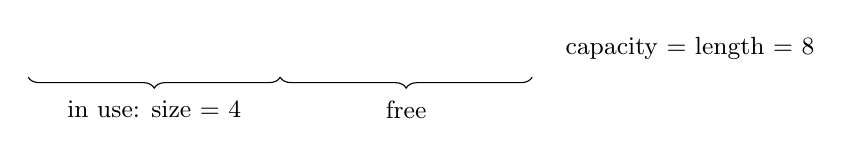
\begin{tikzpicture}
			\hArray[id=v, name={values}, width=0.8, unused={4,...,7}]{40,33,15,27,0,0,0,0}
			\draw[decorate, decoration={brace, mirror, amplitude=4pt}] (0,-0.12) -- (3.2,-0.12)
				node[midway, below=5pt, font=\small] {in use: \hCode{size} = 4};
			\draw[decorate, decoration={brace, mirror, amplitude=4pt}] (3.2,-0.12) -- (6.4,-0.12)
				node[midway, below=5pt, font=\small] {free};
			\node[font=\small, anchor=west] at (6.7,0.25) {capacity = length = 8};
		\end{tikzpicture}
	\end{center}

	\begin{itemize}
		\item A second variable, \hCode{size}, travels with the array
		\item Loops go to \hCode{size}, not to the length
		\item Add at the end: $a[\mathit{size}] \gets x$, then $\mathit{size} \gets \mathit{size} + 1$
		\item Full when $\mathit{size} = \mathit{capacity}$: stop, or grow (\hCode{array1D-3-junior})
	\end{itemize}
\end{frame}
% ~~~~~~~~~~~~~~~~~~~~~~~~~~~~~~~~~~~~~~ A frm




% ~~~~~~~~~~~~~~~~~~~~~~~~~~~~~~~~~~~~~~ V frm
\begin{frame}[t,fragile] \frametitle{Insert and remove}
	\begin{tikzpicture}
		\node[font=\small, anchor=west] at (-0.2,1.05) {\textbf{Insert} 33 at index 1: shift right, \emph{starting from the end}};
		\hArray[id=a, width=0.7, index=below, unused={3,...,5}]{40,15,27,0,0,0}
		\draw[->, colorStop, thick] (a-2.north) to[bend left=60] (a-3.north);
		\draw[->, colorStop, thick] (a-1.north) to[bend left=60] (a-2.north);
		\node at (4.6,0.25) {$\Rightarrow$};
		\hArray[id=b, at={(5.3,0)}, width=0.7, index=below, hot={1}, unused={4,5}]{40,33,15,27,0,0}

		\node[font=\small, anchor=west] at (-0.2,-0.75) {\textbf{Remove} index 0, \emph{keep the order}: shift left};
		\hArray[id=c, at={(0,-1.8)}, width=0.7, index=below, unused={4,5}]{40,33,15,27,0,0}
		\draw[->, colorStop, thick] (c-1.north) to[bend right=60] (c-0.north);
		\draw[->, colorStop, thick] (c-2.north) to[bend right=60] (c-1.north);
		\draw[->, colorStop, thick] (c-3.north) to[bend right=60] (c-2.north);
		\node at (4.6,-1.55) {$\Rightarrow$};
		\hArray[id=d, at={(5.3,-1.8)}, width=0.7, index=below, unused={3,4,5}]{33,15,27,27,0,0}

		\node[font=\small, anchor=west] at (-0.2,-2.55) {\textbf{Remove} index 0, \emph{order does not matter}: move the last one in};
		\hArray[id=e, at={(0,-3.6)}, width=0.7, index=below, unused={4,5}]{40,33,15,27,0,0}
		\draw[->, colorStop, thick] (e-3.north) to[bend right=35] (e-0.north);
		\node at (4.6,-3.35) {$\Rightarrow$};
		\hArray[id=f, at={(5.3,-3.6)}, width=0.7, index=below, hot={0}, unused={3,4,5}]{27,33,15,27,0,0}
	\end{tikzpicture}

	\vspace{0.3em}
	\small Shifting moves up to $n$ elements; moving the last one moves only one.
	Gray cells are outside \hCode{size}: their old values do not matter.
\end{frame}
% ~~~~~~~~~~~~~~~~~~~~~~~~~~~~~~~~~~~~~~ A frm




% ~~~~~~~~~~~~~~~~~~~~~~~~~~~~~~~~~~~~~~ V
\hSection[Methods]{Arrays and methods}
% ~~~~~~~~~~~~~~~~~~~~~~~~~~~~~~~~~~~~~~ A




% ~~~~~~~~~~~~~~~~~~~~~~~~~~~~~~~~~~~~~~ V frm
\begin{frame}[t,fragile] \frametitle{Passing an array passes the arrow}
	\begin{center}
		\begin{tikzpicture}
			\node[draw, rounded corners, gray, minimum width=2.4cm, minimum height=1.0cm, label={[gray, font=\scriptsize]above:caller}] (cf) at (0.6,0.6) {};
			\node[draw, rounded corners, gray, minimum width=2.4cm, minimum height=1.0cm, label={[gray, font=\scriptsize]below:method}] (mf) at (0.6,-1.0) {};
			\node[hvar] (s) at (1.0,0.6) {};
			\node[font=\ttfamily\small, left=2pt of s] {scores};
			\node[hvar] (p) at (1.0,-1.0) {};
			\node[font=\ttfamily\small, left=2pt of p] {a};
			\only<1-2>{\hArray[id=x, at={(4.0,-0.45)}, width=0.8]{70,80,90}}
			\only<3>{\hArray[id=x, at={(4.0,-0.45)}, width=0.8, hot={0,1,2}]{75,85,95}}
			\draw[href] (s.center) -- (x-0.north west);
			\only<1-3>{\draw[href] (p.center) -- (x-0.south west);}
			\only<4>{
				\hArray[id=x, at={(4.0,-0.45)}, width=0.8, hot={0,1,2}]{75,85,95}
				\hArray[id=z, at={(4.0,-1.7)}, width=0.8]{0,0,0}
				\draw[href] (p.center) -- (z-0.west);
			}
		\end{tikzpicture}
	\end{center}

	\begin{itemize}\small
		\item<2-> The parameter \hCode{a} gets a copy of the \emph{arrow}: both refer to one array
		\item<3-> The method changes \hCode{a[i]}: the caller \hEmph{sees} the change
		\item<4-> The method sets \hCode{a} to a new array: only \emph{its own} arrow moves;
		          the caller \hEmph{does not} see it
	\end{itemize}
\end{frame}
% ~~~~~~~~~~~~~~~~~~~~~~~~~~~~~~~~~~~~~~ A frm




% ~~~~~~~~~~~~~~~~~~~~~~~~~~~~~~~~~~~~~~ V frm
\begin{frame}[t,fragile] \frametitle{Returning an array}
	\begin{columns}[T]
		\begin{column}{0.52\textwidth}
			A method can \hEmph{create} an array and return the arrow to it.

			\vspace{0.5em}
			\begin{tikzpicture}
				\hArray[id=x, name={scores}, width=0.8]{75,85,95}
				\hArray[id=y, name={big}, at={(0,-1.2)}, width=0.8, hot={0,1,2}]{150,170,190}
				\draw[->, gray, shorten >=7pt] (x-1.south) -- (y-1.north) node[pos=0.35, right, font=\scriptsize] {$\times 2$};
			\end{tikzpicture}
		\end{column}
		\begin{column}{0.44\textwidth}


% +++++++++++++++++++++++++++++++++++++++ V tbl
%: -Tbl. change or return
\begin{table}
				\small
				\begin{tabular}{@{}L{0.42\textwidth}L{0.50\textwidth}@{}}
					\toprule
					\textbf{Method} & \textbf{Effect} \\
					\midrule
					changes elements   & the caller's array changes \\
					returns a new array & the caller's array stays as it was \\
					\bottomrule
				\end{tabular}
\end{table}%
% +++++++++++++++++++++++++++++++++++++++ A tbl
		\end{column}
	\end{columns}

	\vspace{0.5em}
	\begin{block}{Say which one it is}
		A method that takes an array should say whether it changes it.
		``Returns a new array; \hCode{a} is not changed'' is a good sentence for a comment.
	\end{block}
\end{frame}
% ~~~~~~~~~~~~~~~~~~~~~~~~~~~~~~~~~~~~~~ A frm




% ~~~~~~~~~~~~~~~~~~~~~~~~~~~~~~~~~~~~~~ V
\hSection[Summary]{Summary}
% ~~~~~~~~~~~~~~~~~~~~~~~~~~~~~~~~~~~~~~ A




% ~~~~~~~~~~~~~~~~~~~~~~~~~~~~~~~~~~~~~~ V frm
\begin{frame}[t,fragile] \frametitle{Cheat sheet}


% +++++++++++++++++++++++++++++++++++++++ V tbl
%: -Tbl. cheat sheet
\begin{table}
		\footnotesize
		\begin{tabular}{@{}L{0.22\textwidth}L{0.70\textwidth}@{}}
			\toprule
			\textbf{Idea} & \textbf{Remember} \\
			\midrule
			Array               & many values of one type, under one name, chosen by an index \\
			Index               & $0 \dots n - 1$; the number of elements to skip \\
			Length              & fixed when the array is created; a count, not an index \\
			Default values      & \hCode{0}, \hCode{0.0}, \hCode{false}, code 0, \hCode{null} \\
			Reference           & the variable holds an arrow; \hCode{b = a} copies the arrow (alias) \\
			Copy                & a new array, element by element; \hCode{==} asks ``same array?'' \\
			Traversal patterns  & fill, accumulate, best so far, search, count, transform, filter \\
			Partially filled    & capacity (length) and \hCode{size}; loops go to \hCode{size} \\
			Insert, remove      & shift (keeps order) or move the last one (does not) \\
			Methods             & receive the arrow: may change elements, cannot move the caller's arrow \\
			\bottomrule
		\end{tabular}
\end{table}%
% +++++++++++++++++++++++++++++++++++++++ A tbl
\end{frame}
% ~~~~~~~~~~~~~~~~~~~~~~~~~~~~~~~~~~~~~~ A frm




% ~~~~~~~~~~~~~~~~~~~~~~~~~~~~~~~~~~~~~~ V frm
\begin{frame}[t,fragile] \frametitle{Exercises (paper and pencil)}
	\begin{enumerate}\small
		\item Draw the arrows and the arrays after:
		      \hCode{a} refers to \{4, 5\}; \hCode{b = a}; \hCode{c} is a copy of \hCode{a};
		      \hCode{b[1] = 0}; \hCode{c[0] = 9}. What are \hCode{a[0]} and \hCode{a[1]}?
		\item Trace \emph{IndexOfMax} on \{3, $-2$, 9, 4, 9\}: write $i$ and $b$ after every step.
		      Which 9 is found?
		\item For each question, does it need an array? The smallest value; the second smallest;
		      the values in sorted order; how many values are even.
		\item Write pseudo code for ``the index of the \emph{last} element smaller than $x$, or $-1$''.
		      Is it faster to go from the end?
		\item A partially filled array has capacity 6 and \hCode{size} 4: \{7, 1, 8, 2, \_, \_\}.
		      Draw it after inserting 5 at index 0, then after removing index 2 (keep the order).
		\item Why is $-1$ a good ``not found'' answer, and why would $0$ be a bad one?
	\end{enumerate}
\end{frame}
% ~~~~~~~~~~~~~~~~~~~~~~~~~~~~~~~~~~~~~~ A frm




% ~~~~~~~~~~~~~~~~~~~~~~~~~~~~~~~~~~~~~~ V frm
\begin{frame}[t,fragile] \frametitle{Where to go next}


% +++++++++++++++++++++++++++++++++++++++ V tbl
%: -Tbl. decks
\begin{table}
		\small
		\begin{tabular}{@{}L{0.30\textwidth}L{0.62\textwidth}@{}}
			\toprule
			\textbf{Deck} & \textbf{What it adds} \\
			\midrule
			\hCode{array1D-5-examples}  & every idea of this deck as a small Java program \\
			\hCode{array1D-1-freshman}  & Java syntax, the common errors and how to read them \\
			\hCode{array1D-2-sophomore} & \hCode{java.util.Arrays}, tests, input, good habits \\
			\hCode{array1D-3-junior}    & growing, searching, sorting, performance \\
			\hCode{array1D-4-senior}    & inside the JVM, security, production use \\
			\hCode{arrayND}             & arrays of arrays: tables, grids, images \\
			\bottomrule
		\end{tabular}
\end{table}%
% +++++++++++++++++++++++++++++++++++++++ A tbl


	\vspace{0.5em}
	\small Reading: bjlo2, Chapter 6 (arrays); The Java Tutorials, Arrays \cite{TheJavaTutorialsArray}.
\end{frame}
% ~~~~~~~~~~~~~~~~~~~~~~~~~~~~~~~~~~~~~~ A frm




% ~~~~~~~~~~~~~~~~~~~~~~~~~~~~~~~~~~~~~~ V frm
\begin{frame}[t,fragile] \frametitle{References}
	\setbeamertemplate{bibliography item}[text]
	\bibliographystyle{IEEEtran}
	\tiny\bibliography{../../hblib/hblibDataStructures}
\end{frame}
% ~~~~~~~~~~~~~~~~~~~~~~~~~~~~~~~~~~~~~~ A frm




% ~~~~~~~~~~~~~~~~~~~~~~~~~~~~~~~~~~~~~~ V frm
\begin{frame}[t,fragile]
	\begin{center}
		\vspace{4cm}
		\hRemark{\Huge Questions?}
	\end{center}
\end{frame}
% ~~~~~~~~~~~~~~~~~~~~~~~~~~~~~~~~~~~~~~ A frm



\end{document}
